\documentclass[a4j, 10pt, titlepage]{jsarticle}

\usepackage{izumin}
\usepackage{listings}
\lstset{
    language={Ruby},
    frame=shadowbox,
    numbers=left,
    basicstyle={\small}
}

\begin{document}

\title{数値計算法 課題}
\author{ME1301 泉 将之}
\date{\today}
\maketitle

% ================================================================

\section*{微分方程式の数値解}

\eqn{\dd{x}{t} = (\cos t) x (2 - x)}
\eqn{x(0) = 1}

\lstinputlisting[label=src:ivp, caption=initial\_value\_problem\_solver.rb]{src/initial_value_problem_solver.rb}
\lstinputlisting[label=src:calcmethod, caption=calc\_method.rb]{src/calc_method.rb}
\lstinputlisting[label=src:q1, caption=q1.rb]{src/q1.rb}

\fig{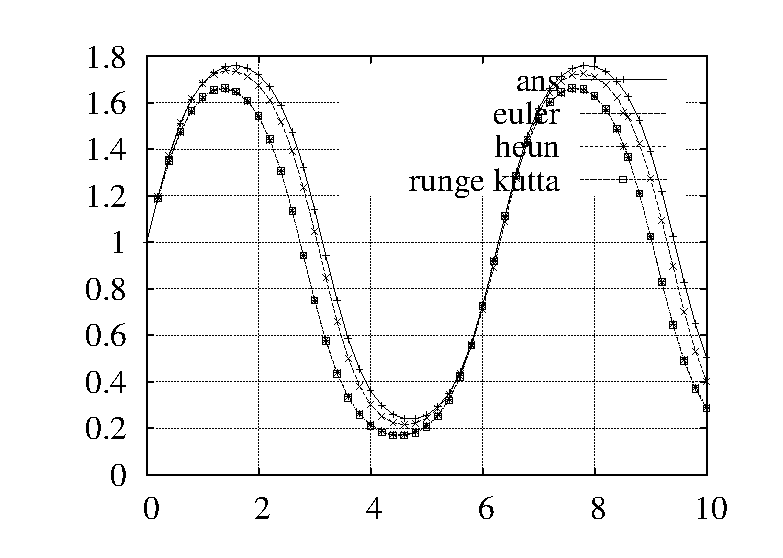
\includegraphics[width=120mm]{img/q1-1.eps}}{Euler法,Heunの矩形公式,4次Runge-Kutta法の厳密解との比較}{q1-1}
\fig{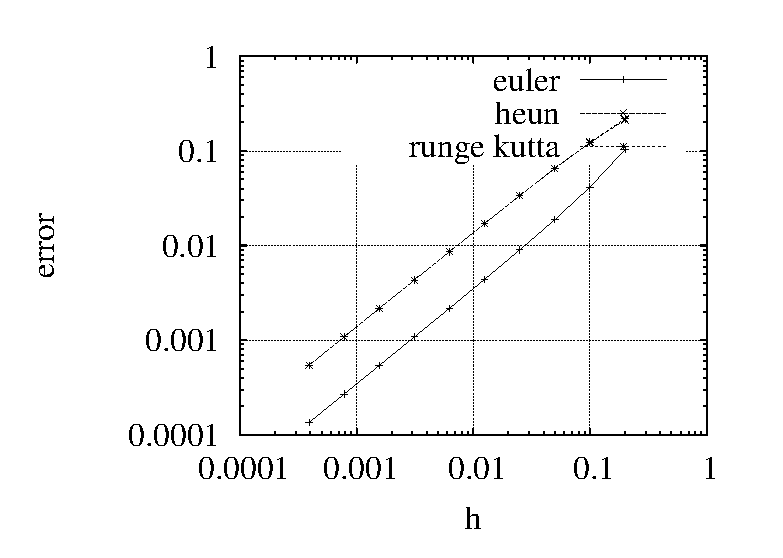
\includegraphics[width=120mm]{img/q1-2.eps}}{Euler法,Heunの矩形公式,4次Runge-Kutta法の厳密解との誤差}{q1-2}

% ================================================================

\section*{連立微分方程式の数値解}

\eqn{
    \begin{cases}
        \dd{x}{t} &= - \sigma x + \sigma y \\
        \dd{y}{t} &= rx - y - xz \\
        \dd{z}{t} &= -bz + xy
    \end{cases}
}
\eqn{\sigma = 10,~ r = 28,~ b = \frac{8}{3}}
\eqn{x(0) = 0,~ y(0) = 1.1,~ z(0) = 0}

\lstinputlisting[label=src:q2, caption=q2.rb]{src/q2.rb}

\fig{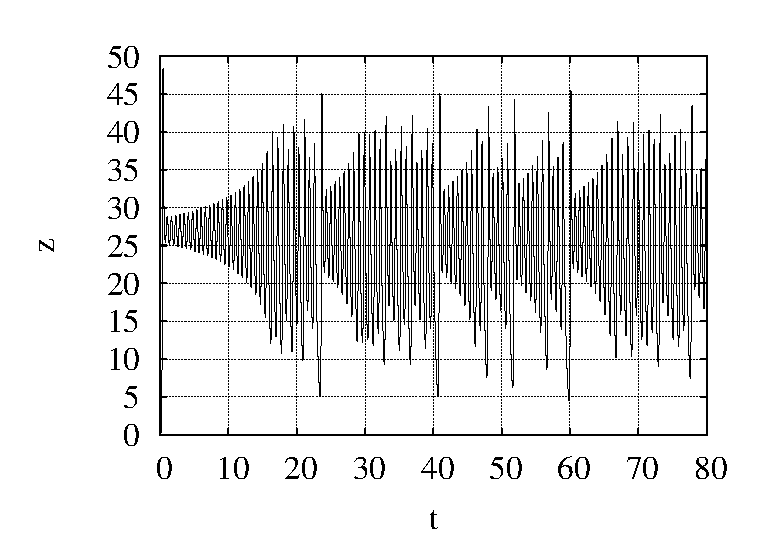
\includegraphics[width=120mm]{img/q2-tz.eps}}{4次Runge-Kutta法による数値解のtz-図}{q2-tz}
\fig{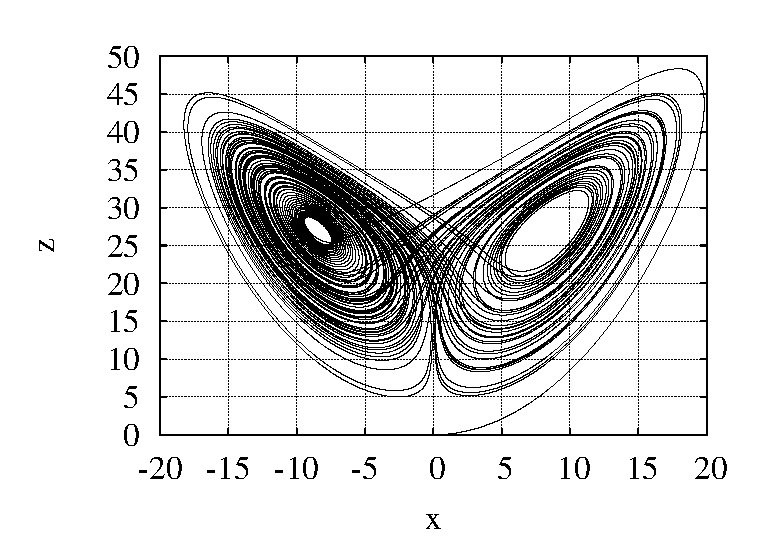
\includegraphics[width=120mm]{img/q2-xz.eps}}{4次Runge-Kutta法による数値解のxz-図}{q2-xz}
\fig{\includegraphics[width=120mm]{img/q2-xyz.eps}}{4次Runge-Kutta法による数値解のxyz-図}{q2-xyz}
\fig{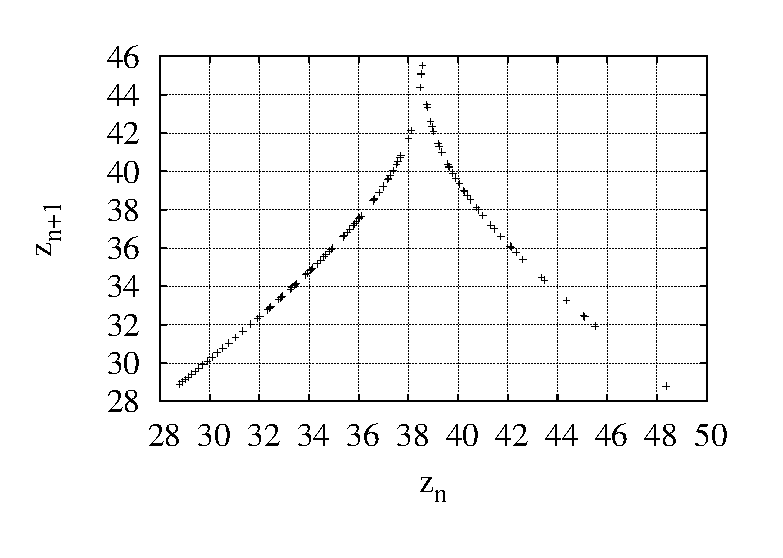
\includegraphics[width=120mm]{img/q2-lorenz_map.eps}}{zの極大値によるLorenz map}{q2-lmap}

% ================================================================

\section*{時系列データのパワースペクトル}

\eqn{
    f(t) =
    \begin{cases}
        \frac{1}{2} (\cos \omega t)^3 & (0 \leq x \leq 2L) \\
        0 & (t < 0,~ t > 2L)
    \end{cases}
}
\eqn{\omega = 5.026548,~ L = 25}
\lstinputlisting[label=src:q3, caption=q3.rb]{src/q3.rb}

\end{document}